\section{Durchführung}
\label{sec:Durchführung}

\subsection{Bauteile und Aufbau}
\label{sec:d1}
Der Versuch ist in zwei Teile geteilt, für jeden werden andere Utensilien 
benötigt. Für den Teil aus \autoref{sec:d2} werden zunächst nur die Komponenten 
des oberen Bildabschnitts aus \autoref{fig:d1} verwendet. Dazu gehören 
8 Zylinder von $\qty{7.5}{\centi\meter}$ und 12 Zylinder mit einer Länge von 
$\qty{5}{\centi\meter}$. Für \autoref{sec:d3} sind lediglich die Kugelresonatoren 
und die Ringe relevant. Diese befinden sich in \autoref{fig:d1} mittig und unten 
rechts. Es handelt sich um zwei Kugelhälften, welche gegenüberliegend mit
Mikrofon und Lautsprecher ausgestattet sind. Sie werden für das Experiment 
aufeinander gesetzt. An der oberen Hälfte sind ringsum Gradmaße aufgetragen,
auf der unteren Hälfte befindet sich eine Einkerbung. So können 
Mikrofon und Lautsprecher in beliebigen Winkeln zueinander ausgerichtet werden.
\begin{figure}[H]
    \centering
        \centering
        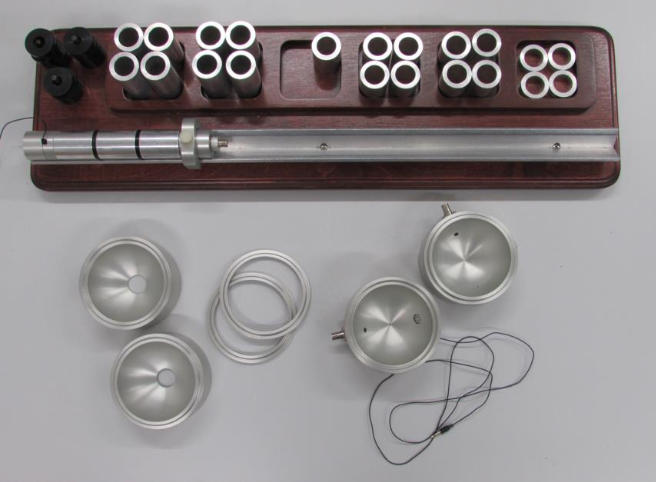
\includegraphics[width=0.75\textwidth]{Bilder/bauteile.png}
        \caption{Resonatoren in Zylinderform verschiedener Größen und 
        Kugelresonatoren inklusive Ringe. \cite{anleitung15}}
    \hfill
    \label{fig:d1}
\end{figure}
\noindent Neben den Komponenten der Resonatoren steht auch ein Computer und 
ein Oszilloskop mit Sinusgenerator zur Verfügung. Letzteres wird für diesen 
Versuch jedoch nicht genutzt, jegliche Datensätze werden mit dem Computer 
aufgenommen. Angeschlossen wird alles wie in \autoref{fig:d2} dargestellt.
\begin{figure}[H]
    \centering
        \centering
        
\includegraphics[width=0.75\textwidth]{Bilder/schaltplan.png}
        \caption{Schaltplan für die Steuerung, die Hohlraumresonatoren und 
        das Oszilloskop \cite{anleitung15}}
    \hfill
    \label{fig:d2}
\end{figure}
\noindent Ein Bild des vollständigen Aufbaus ist in \autoref{fig:d3} zu sehen.
Im Vordergrund sind (links) die Resonatoren zu erkennen, dabei wurde der 
Kugelresonator bereits zusammengesetzt. Rechts der Computer, auf dem mithilfe
des Programms ``SpectrumSLC'' die Druckamplituden in Abhängigkeit der Frequenz 
gemessen werden.
\begin{figure}[H]
    \centering
        \centering
        
\includegraphics[width=0.8\textwidth]{Bilder/aufbau.jpg}
        \caption{Bild des vollständigen Aufbaus samt aller Komponenten. (Eigenaufnahme)}
    \hfill
    \label{fig:d3}
\end{figure}

\subsection{Die Vorbereitung}
\label{sec:d2}
Die Messung wird mit einem $\qty{7.5}{\centi\meter}$ langen Zylinder begonnen, 
dieser wird auf die dafür vorgesehene Schiene gelegt und das Mikrofon so
herangeschoben, dass alle Teile möglichst verlustfrei verbunden sind. Am 
Computer wird daraufhin das Verhältnis von Amplitude und Frequenz in einem 
Bereich von $\qty{100}{\hertz}$ bis $\qty{12}{\kilo\hertz}$ gemessen und
anschließend in Form von Rohdaten gespeichert. Dabei wird das Spektrum in 
$\qty{10}{\hertz}$-Schritten abgefahren, das Programm mittelt die gemessenen 
Werte über $\qty{50}{\milli\second}$ hinweg. Als nächstes wird ein weiterer
Zylinder eingebaut bis eine Anzahl von acht erreicht ist. Für jede Kette an
Zylindern wird der soeben beschriebene Messvorgang wiederholt.
\\
Das gleiche geschieht auch für die Zylinder von $\qty{5}{\centi\meter}$ Länge, 
da es von diesen zwölf gibt, wird die Messung dementsprechend oft wiederholt.

\subsection{Das Wasserstoffatom}
\label{sec:d3}
Für die Messungen an dem Kugelresonator zur Simulation des Wasserstoffatoms 
wird zunächst der Resonator an den Computer angeschlossen. Bei einem Winkel 
von 180° zwischen Mikrofon und Lautsprecher wird bei $\qty{5}{\hertz}$-Schritten 
(und $\qty{50}{\milli\second}$ pro Schritt) das Spektrum von $\qty{100}{\hertz}$ 
bis $\qty{12}{\kilo\hertz}$ erfasst. \\
Im nächsten Teil werden spezifische Peaks des Spektrums untersucht. Für die 
Peaks bei $\qty{2.3}{\kilo\hertz}$, $\qty{3.7}{\kilo\hertz}$, $\qty{5}{\kilo\hertz}$
und $\qty{7.4}{\kilo\hertz}$ werden in einem Bereich von $\pm \qty{0.2}{\kilo\hertz}$
um die zu untersuchenden Stelle Druckamplituden gemessen. Für alle vier Peaks 
werden winkelabhängige Messungen gemacht, angefangen bei 0° wird in 5°-Schritten
das zu untersuchende Spektrum bishin zu 180° zwischen dem Mikrofon und Lautsprecher 
abgetastet. \\
Für ein Spektrum von $\qty{1.8}{\kilo\hertz}$ bis $\qty{2.6}{\kilo\hertz}$ wird 
bei einer Schrittweite von $\qty{1}{\hertz}$ (und gleicher Zeiteinstellung von 
$\qty{50}{\milli\second}$ pro Schritt) die Messung für 180° wiederholt. Der 
Unterschied besteht darin, dass nun die Ringe eingebaut werden. Diese sind 
$\qty{3}{\milli\meter}$ und $\qty{6}{\milli\meter}$ dick. Anschließend werden
beide Ringe überlappend eingesetzt. Die Amplituden werden im genannten Spektrum 
mit der Winkelmessung wie zuvor untersucht.